% \subsection{Sections on the three body problem we did not use}

% \subsubsection{Three-Body Problem}
% The three-body problem, originating with Isaac Newton's *Principia Mathematica* in 1687 \cite{newton1687principia}, involves predicting the motion of three celestial bodies interacting under mutual gravitational attraction. Newton first addressed the mutual gravitational influences of Earth, the Moon, and the Sun, laying the foundation for this field of study. The term "three-body problem" was first used during the competitive analyses of Jean le Rond d'Alembert and Alexis Clairaut in Paris in 1747 \cite{dalembert1747}. 
% The gravitational interactions of the three-bodies are governed by Newton's law of universal gravitation and Newton's second law of motion. The differential equations describing the motion of each body are derived from these principles. For bodies \(i\), \(j\), with positions \( \mathbf{r}_i \) and \( \mathbf{r}_j \), and masses \(m_i\) and \(m_j\), the acceleration \( \mathbf{a}_i \) of body \(i\) due to \(j\) is given by:

% \begin{equation}
%     m_i \ddot{\mathbf{r}}_i = \sum_{\substack{j=1 \\ j \neq i}}^3 G \frac{m_i m_j (\mathbf{r}_j - \mathbf{r}_i)}{|\mathbf{r}_j - \mathbf{r}_i|^3},
% \end{equation}
% where \(G = 6.67430 \times 10^{-11}\) \si{m^{3}.kg^{-1}.s^{-2}} is the gravitational constant. The masses of the three bodies used in this experiment are set to replicate those of the triple star system Alpha Centauri located in the southern constellation of Centaurus about \(4.2465\) light-years away. These masses are multiplicities of our sun's mass \(m_s \coloneq 1.989 \times 10^{30}\) \si{kg}. Thus, we have that \(m_1 = 1.1\cdot m_s\), \(m_2 = 0.907\cdot m_s\) and \(m_3 = 0.123\cdot m_s\).


% \begin{figure}
%     \centering
%         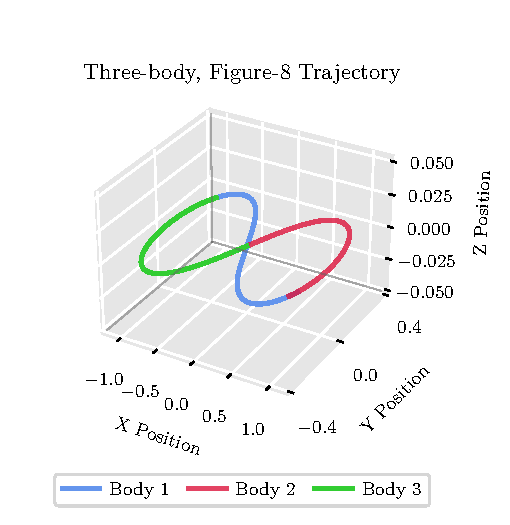
\includegraphics[width=0.48\textwidth]{project_2/images/three_body_figure8.pdf}
%         \label{fig:threebody}
%          \caption{Figure 8 Trajectory of a Three-Body System with Equal Masses: This plot shows the trajectories resulting from a stable figure-8 configuration in the three-body problem. The initial conditions were meticulously selected to test the robustness and accuracy of numerical solvers in replicating known stable solutions.}
%     \label{fig:init_dynamical_systems}
% \end{figure}





    
% \paragraph{Bounds for Initial Conditions}
% Below are the bounds for each variable used in the simulations:

% \begin{table}[h!]
% \centering
% \begin{tabular}{ccc}
% \toprule
% \textbf{System} & \textbf{Variable} & \textbf{Bounds} \\
% \midrule
% \multirow{3}{*}{Lorenz System} & \(z_1\) & \([-36, 36]\) \\
%                                & \(z_2\) & \([-48, 48]\) \\
%                                & \(z_3\) & \([-16, 66]\) \\
% \midrule
% \multirow{3}{*}{Three-body Problem} & \parbox{2cm}{Position \\ \((x, y, z)\)} & \([-10^6, 10^6]\) m \\[1.2em]
%                                     & \parbox{2cm}{Velocity \\ \((v_x, v_y, v_z)\)} & \([-3 \times 10^4, 3 \times 10^4]\) m/s \\
% \bottomrule
% \end{tabular}
% \caption{Initial condition bounds for the Lorenz system and the Three-body problem.}
% \label{tab:bounds}
% \end{table}

% \paragraph{Sampling Method: Latin Hypercube Sampling}

% Latin Hypercube Sampling (LHS) is used to generate initial conditions for the Lorenz system and three body problem. By dividing each variable's range into equal, non-overlapping intervals and randomly selecting a sample from each interval, LHS ensures a comprehensive and uniform exploration of the parameter space. This method significantly enhances the diversity of the simulation data, reducing sampling bias and improving the estimates of system responses \cite{mckay1979comparison, helton2003latin}. Consequently, the autoencoder SINDy framework benefits from a robust dataset, enabling it to effectively learn and predict the dynamics across varied initial conditions.\\

% On the other hand, the Figure-8 trajectory in the Three-Body Problem, with its initial conditions set to a specific symmetrical pattern and normalized masses and gravitational constant \cite{moore1993braids}, requires precise and stable numerical integration to maintain the periodicity and stability of the orbit. The accuracy and adaptive step sizing feature of RK45 is crucial here.

%  Figure \ref{fig:init_dynamical_systems} illustrates these dynamics, showcasing both the chaotic trajectories of the Lorenz system and the periodic orbits of the Three-Body Problem.\\

 
% These simulations test the solver's capabilities in handling distinct dynamical behaviors and also serve as benchmarks for validating the numerical integration approach used in our study. By ensuring that the solver reproduces the well-documented dynamics of these systems, we can confidently use these models to further explore and analyze the behavior of similar systems.


% \subsubsection{High-Dimensional Data Transformation Using Legendre Polynomials}\label{subsec:high-dim-data-transform}

% The transformation of "low"-dimensional simulated data into a high-dimensional space using Legendre polynomials is central to testing the effectiveness of the autoencoder SINDy framework. This method allows us to assess the framework's ability to reconstruct low-dimensional dynamics and reveal the fundamental laws that govern these systems from complex, high-dimensional datasets, thereby verifying its robustness and adaptability \cite{Champion_2019}.

% \paragraph{Transformation Implementation}
% Legendre polynomials are employed for their orthogonality properties and their capacity to represent complex functions within a bounded interval effectively. These characteristics make them ideal for transforming trajectory data from dynamical systems into high-dimensional polynomial spaces, enriching the feature space and providing a stringent test for the autoencoder's decoding capabilities. Below is the pseudocode outlining the computational steps involved in this process:

% \begin{algorithm}
% \caption{Generation of High-Dimensional Datasets from Dynamical Systems}
% \label{alg:high_dim_data_generation}
% \begin{algorithmic}[1]
% \Require Number of initial conditions (\texttt{num\_initial\_conditions}), number of time steps (\texttt{n\_steps}), dimension before transformation (\texttt{dim}), and dimension after transformation (\texttt{high\_dim})

% \State \texttt{solutions} $\gets$ array of dimensions (\texttt{num\_initial\_conditions}, \texttt{n\_steps}, \texttt{dim}) \Comment{Array to store ODE solutions}
% \State \texttt{high\_dim\_data\_array} $\gets$ array of dimensions (\texttt{num\_initial\_conditions}, \texttt{n\_steps}, \texttt{high\_dim}) \Comment{Array for transformed data}

% \State \texttt{initial\_conditions} $\gets$ Sample initial conditions within \texttt{bounds} using LHS
% \State \texttt{modes} $\gets$ Evaluate \texttt{num\_modes} Legendre polynomials across a uniformly spaced domain within $[-1, 1]$ at \texttt{high\_dim} points

% \For{each initial condition in \texttt{initial\_conditions}}
%     \State \texttt{solution} $\gets$ Solve ODE for the current initial condition
%     \State Store \texttt{solution} in \texttt{solutions} array
%     \If{\texttt{high\_dim\_trans}}
%         \For{each mode \texttt{idx} and each time step \texttt{j} in \texttt{solution}}
%             \State \texttt{mod\_idx} $\gets$ \texttt{idx} mod dimension of \texttt{solution}
%             \If{\texttt{idx} $<$ dimension of \texttt{solution}}
%                 \State \texttt{term} $\gets$ \texttt{modes[idx]} * \texttt{solution[j, mod\_idx]}
%             \Else
%                 \State \texttt{term} $\gets$ \texttt{modes[idx]} * \texttt{solution[j, mod\_idx]} ** 3 %\Comment{Nonlinear transformation}
%             \EndIf
%             \State \texttt{high\_dim\_data\_array[i, j]} $\gets$ \texttt{term}
%         \EndFor
%     \EndIf
% \EndFor
% \end{algorithmic}
% \end{algorithm}

% \paragraph{Transformation Formula for Lorenz and Three-Body Systems}
% For the Lorenz system, the transformation is represented as:

% \begin{align*}
%     \mathbf{D}(t) = &\mathbf{P}_1\mathbf{S}_1(t) + \mathbf{P}_2\mathbf{S}_2(t) + \mathbf{P}_3\mathbf{S}_3(t) + \\ &\mathbf{P}_4\mathbf{S}_1(t)^3 + \mathbf{P}_5\mathbf{S}_2(t)^3 + \mathbf{P}_6\mathbf{S}_3(t)^3,
% \end{align*}
% and similarly for the three-body problem, illustrating the detailed data transformation undertaken for each system.


% \subsection{Three-Body Data}
% The data generation for the three-body simulation involves several steps, outlined in the Python class \texttt{ThreeBodyData}. The process includes setting up the governing differential equations, sampling a large amount of diffrenent initial conditions, and solving the equations by numerical integrating, before transforming the solution into a high-dimensional data set. This creates a large array of differnet high-dimensional simulations that the autoencoder-SINDy model can train on.
% \subsubsection{Derivation of the Governing Three-Body Equations}



% % The gravitational interactions in a three-body system are governed by Newton's law of universal gravitation and Newton's second law of motion. The differential equations describing the motion of each body are derived from these principles. For bodies \(i\), \(j\), with positions \( \mathbf{r}_i \) and \( \mathbf{r}_j \), and masses \(m_i\) and \(m_j\), the acceleration \( \mathbf{a}_i \) of body \(i\) due to \(j\) is given by:
% % \begin{equation}
% %     \mathbf{a}_i = -G \sum_{j \neq i} \frac{m_j (\mathbf{r}_i - \mathbf{r}_j)}{|\mathbf{r}_i - \mathbf{r}_j|^3}
% % \end{equation}
% % where \(G = 6.67430 \times 10^{-11}\) \si{m^{3}.kg^{-1}.s^{-2}} is the gravitational constant.
% The motion of three bodies under mutual gravitational attraction can be modeled by applying Newton's law of universal gravitation combined with Newton's second law of motion. The equations describe the acceleration of each body as a result of the gravitational forces exerted by the other two bodies in the system.\\

% Consider three bodies with masses \(m_1\), \(m_2\), and \(m_3\) located at positions \(\mathbf{r}_1\), \(\mathbf{r}_2\), and \(\mathbf{r}_3\) respectively. The force on any body \(i\) due to body \(j\) is given by Newton's law of universal gravitation:
% \begin{equation}
% \mathbf{F}_{ij} = -G \frac{m_i m_j}{|\mathbf{r}_i - \mathbf{r}_j|^3} (\mathbf{r}_i - \mathbf{r}_j),
% \end{equation}
% where \(G\) is the gravitational constant.\\
% The total force on each body is the vector sum of the forces exerted by the other two bodies:
% \begin{align}
% \mathbf{F}_1 &= \mathbf{F}_{12} + \mathbf{F}_{13}, \\
% \mathbf{F}_2 &= \mathbf{F}_{21} + \mathbf{F}_{23}, \\
% \mathbf{F}_3 &= \mathbf{F}_{31} + \mathbf{F}_{32}.
% \end{align}

% Substituting the force definition, we have:
% \begin{small}
% \begin{align}
% \mathbf{F}_1 &= -G \left( \frac{m_1 m_2}{|\mathbf{r}_1 - \mathbf{r}_2|^3} (\mathbf{r}_1 - \mathbf{r}_2) + \frac{m_1 m_3}{|\mathbf{r}_1 - \mathbf{r}_3|^3} (\mathbf{r}_1 - \mathbf{r}_3) \right), \\
% \mathbf{F}_2 &= -G \left( \frac{m_2 m_1}{|\mathbf{r}_2 - \mathbf{r}_1|^3} (\mathbf{r}_2 - \mathbf{r}_1) + \frac{m_2 m_3}{|\mathbf{r}_2 - \mathbf{r}_3|^3} (\mathbf{r}_2 - \mathbf{r}_3) \right), \\
% \mathbf{F}_3 &= -G \left( \frac{m_3 m_1}{|\mathbf{r}_3 - \mathbf{r}_1|^3} (\mathbf{r}_3 - \mathbf{r}_1) + \frac{m_3 m_2}{|\mathbf{r}_3 - \mathbf{r}_2|^3} (\mathbf{r}_3 - \mathbf{r}_2) \right).
% \end{align}
% \end{small}

% Applying Newton's second law \(\mathbf{F} = m\mathbf{a}\), the accelerations are:
% \begin{align}
% \mathbf{a}_1 &= \frac{\mathbf{F}_1}{m_1}, \label{eq:a1} \\
% \mathbf{a}_2 &= \frac{\mathbf{F}_2}{m_2}, \label{eq:a2} \\
% \mathbf{a}_3 &= \frac{\mathbf{F}_3}{m_3}. \label{eq:a3}
% \end{align}

% These derived equations allow for the calculation of the positions and velocities of the bodies in a three-body system through numerical methods, given initial conditions.


% \subsubsection{Initial Conditions}
% Initial conditions critically influence the system's evolution and dynamics. Since the governing equations \(\ref{eq:a1}\), \(\ref{eq:a2}\), and \(\ref{eq:a3}\) are second ordered ordinary differential equations two initial conditions per equation are needed for the numerical integration. Therefore, we sample the initial positions and velocities of each body within bounded cubes in \(\mathbb{R}^3\), \([0,10^{11}]^3\) and \([-20^4, 20^4]^3\) respectively, using a uniform distribution to ensure a broad exploration. Random sampling from these distributions helps in providing comprehensive coverage of possible system states, which is crucial for studying the chaotic nature of the three-body problem.

% The masses of the bodies are set as multiplicities of our sun's mass, \(m_s \coloneq 1.989 \times 10^{30}\) \si{kg}. Thus, we have that \(m_1 = 1.1\cdot m_s\), \(m_2 = 0.907\cdot m_s\) and \(m_3 = 0.123\cdot m_s\).

% \subsubsection{Numerical Integration}
% The system of differential equations is solved using the \texttt{solve\_ivp} method from the \texttt{scipy.integrate} library \cite{scipy_solve_ivp}, which implements the Runge-Kutta 45 (RK45) method. The RK45 is an explicit Runge-Kutta method of order 5(4), as detailed in the work by Dormand and Prince \cite{dormand1980family}. This notation indicates that the method employs a fifth-order Runge-Kutta formula for the step integration but controls the error using a fourth-order formula, thus balancing computational efficiency with precision in numerical integration. Additionally, a quartic interpolation polynomial is used to generate a dense output \cite{shampine1986some}.


%CHAT-GPT-fraser
%Numerical integration plays a pivotal role in solving the systems of differential equations that govern the dynamics of both the Lorenz system and the Three-Body Problem. 
%is particularly well-suited for our purpose due to its 
%particularly
%